% Options for packages loaded elsewhere
\PassOptionsToPackage{unicode}{hyperref}
\PassOptionsToPackage{hyphens}{url}
%
\documentclass[
]{article}
\usepackage{lmodern}
\usepackage{amsmath}
\usepackage{ifxetex,ifluatex}
\ifnum 0\ifxetex 1\fi\ifluatex 1\fi=0 % if pdftex
  \usepackage[T1]{fontenc}
  \usepackage[utf8]{inputenc}
  \usepackage{textcomp} % provide euro and other symbols
  \usepackage{amssymb}
\else % if luatex or xetex
  \usepackage{unicode-math}
  \defaultfontfeatures{Scale=MatchLowercase}
  \defaultfontfeatures[\rmfamily]{Ligatures=TeX,Scale=1}
\fi
% Use upquote if available, for straight quotes in verbatim environments
\IfFileExists{upquote.sty}{\usepackage{upquote}}{}
\IfFileExists{microtype.sty}{% use microtype if available
  \usepackage[]{microtype}
  \UseMicrotypeSet[protrusion]{basicmath} % disable protrusion for tt fonts
}{}
\makeatletter
\@ifundefined{KOMAClassName}{% if non-KOMA class
  \IfFileExists{parskip.sty}{%
    \usepackage{parskip}
  }{% else
    \setlength{\parindent}{0pt}
    \setlength{\parskip}{6pt plus 2pt minus 1pt}}
}{% if KOMA class
  \KOMAoptions{parskip=half}}
\makeatother
\usepackage{xcolor}
\IfFileExists{xurl.sty}{\usepackage{xurl}}{} % add URL line breaks if available
\IfFileExists{bookmark.sty}{\usepackage{bookmark}}{\usepackage{hyperref}}
\hypersetup{
  pdftitle={MSc. Research Methods - Statistikteil Loesungen Beispiel},
  pdfauthor={Juergen Dengler},
  hidelinks,
  pdfcreator={LaTeX via pandoc}}
\urlstyle{same} % disable monospaced font for URLs
\usepackage[margin=1in]{geometry}
\usepackage{color}
\usepackage{fancyvrb}
\newcommand{\VerbBar}{|}
\newcommand{\VERB}{\Verb[commandchars=\\\{\}]}
\DefineVerbatimEnvironment{Highlighting}{Verbatim}{commandchars=\\\{\}}
% Add ',fontsize=\small' for more characters per line
\usepackage{framed}
\definecolor{shadecolor}{RGB}{248,248,248}
\newenvironment{Shaded}{\begin{snugshade}}{\end{snugshade}}
\newcommand{\AlertTok}[1]{\textcolor[rgb]{0.94,0.16,0.16}{#1}}
\newcommand{\AnnotationTok}[1]{\textcolor[rgb]{0.56,0.35,0.01}{\textbf{\textit{#1}}}}
\newcommand{\AttributeTok}[1]{\textcolor[rgb]{0.77,0.63,0.00}{#1}}
\newcommand{\BaseNTok}[1]{\textcolor[rgb]{0.00,0.00,0.81}{#1}}
\newcommand{\BuiltInTok}[1]{#1}
\newcommand{\CharTok}[1]{\textcolor[rgb]{0.31,0.60,0.02}{#1}}
\newcommand{\CommentTok}[1]{\textcolor[rgb]{0.56,0.35,0.01}{\textit{#1}}}
\newcommand{\CommentVarTok}[1]{\textcolor[rgb]{0.56,0.35,0.01}{\textbf{\textit{#1}}}}
\newcommand{\ConstantTok}[1]{\textcolor[rgb]{0.00,0.00,0.00}{#1}}
\newcommand{\ControlFlowTok}[1]{\textcolor[rgb]{0.13,0.29,0.53}{\textbf{#1}}}
\newcommand{\DataTypeTok}[1]{\textcolor[rgb]{0.13,0.29,0.53}{#1}}
\newcommand{\DecValTok}[1]{\textcolor[rgb]{0.00,0.00,0.81}{#1}}
\newcommand{\DocumentationTok}[1]{\textcolor[rgb]{0.56,0.35,0.01}{\textbf{\textit{#1}}}}
\newcommand{\ErrorTok}[1]{\textcolor[rgb]{0.64,0.00,0.00}{\textbf{#1}}}
\newcommand{\ExtensionTok}[1]{#1}
\newcommand{\FloatTok}[1]{\textcolor[rgb]{0.00,0.00,0.81}{#1}}
\newcommand{\FunctionTok}[1]{\textcolor[rgb]{0.00,0.00,0.00}{#1}}
\newcommand{\ImportTok}[1]{#1}
\newcommand{\InformationTok}[1]{\textcolor[rgb]{0.56,0.35,0.01}{\textbf{\textit{#1}}}}
\newcommand{\KeywordTok}[1]{\textcolor[rgb]{0.13,0.29,0.53}{\textbf{#1}}}
\newcommand{\NormalTok}[1]{#1}
\newcommand{\OperatorTok}[1]{\textcolor[rgb]{0.81,0.36,0.00}{\textbf{#1}}}
\newcommand{\OtherTok}[1]{\textcolor[rgb]{0.56,0.35,0.01}{#1}}
\newcommand{\PreprocessorTok}[1]{\textcolor[rgb]{0.56,0.35,0.01}{\textit{#1}}}
\newcommand{\RegionMarkerTok}[1]{#1}
\newcommand{\SpecialCharTok}[1]{\textcolor[rgb]{0.00,0.00,0.00}{#1}}
\newcommand{\SpecialStringTok}[1]{\textcolor[rgb]{0.31,0.60,0.02}{#1}}
\newcommand{\StringTok}[1]{\textcolor[rgb]{0.31,0.60,0.02}{#1}}
\newcommand{\VariableTok}[1]{\textcolor[rgb]{0.00,0.00,0.00}{#1}}
\newcommand{\VerbatimStringTok}[1]{\textcolor[rgb]{0.31,0.60,0.02}{#1}}
\newcommand{\WarningTok}[1]{\textcolor[rgb]{0.56,0.35,0.01}{\textbf{\textit{#1}}}}
\usepackage{graphicx}
\makeatletter
\def\maxwidth{\ifdim\Gin@nat@width>\linewidth\linewidth\else\Gin@nat@width\fi}
\def\maxheight{\ifdim\Gin@nat@height>\textheight\textheight\else\Gin@nat@height\fi}
\makeatother
% Scale images if necessary, so that they will not overflow the page
% margins by default, and it is still possible to overwrite the defaults
% using explicit options in \includegraphics[width, height, ...]{}
\setkeys{Gin}{width=\maxwidth,height=\maxheight,keepaspectratio}
% Set default figure placement to htbp
\makeatletter
\def\fps@figure{htbp}
\makeatother
\setlength{\emergencystretch}{3em} % prevent overfull lines
\providecommand{\tightlist}{%
  \setlength{\itemsep}{0pt}\setlength{\parskip}{0pt}}
\setcounter{secnumdepth}{-\maxdimen} % remove section numbering
\ifluatex
  \usepackage{selnolig}  % disable illegal ligatures
\fi

\title{MSc. Research Methods - Statistikteil Loesungen Beispiel}
\author{Juergen Dengler}
\date{Oktober 2020}

\begin{document}
\maketitle

\hypertarget{musterloesung-beispiel}{%
\subsection{Musterloesung Beispiel}\label{musterloesung-beispiel}}

\href{14_Statistik2/RFiles/Loesung_Beispiel_v.01.R}{RCode als
Download}\\
\href{Statistik_Übungslösung_Beispiel.pdf}{Loesungstext Beispiel}

\textbf{Übungsaufgabe (hier so ausführlich formuliert, wie dies auch in
der Klausur der Fall sein wird)}

\begin{itemize}
\tightlist
\item
  Laden Sie den Datensatz decay.csv. Dieser enthält die Zahl
  radioaktiver Zerfälle pro Zeiteinheit (amount) für Zeitpunkte (time)
  nach dem Start des Experimentes.
\item
  \textbf{Ermitteln Sie ein statistisches Modell, dass die
  Zerfallshäufigkeit in Abhängigkeit von der Zeit beschreibt.}
\item
  Bitte erklären und begründen Sie die einzelnen Schritte, die Sie
  unternehmen, um zu diesem Ergebnis zu kommen. Dazu erstellen Sie bitte
  ein Word-Dokument, in das Sie Schritt für Schritt den verwendeten
  R-Code, die dazu gehörigen Ausgaben von R, Ihre Interpretation
  derselben und die sich ergebenden Schlussfolgerungen für das weitere
  Vorgehen dokumentieren.
\item
  Dieser Ablauf sollte insbesondere beinhalten:

  \begin{itemize}
  \tightlist
  \item
    Überprüfen der Datenstruktur nach dem Einlesen, welches sind die
    abhängige(n) und welches die unabängige(n) Variablen
  \item
    Explorative Datenanalyse, um zu sehen, ob evtl. Dateneingabefehler
    vorliegen oder Datentransformationen vorgenommen werden sollten
  \item
    Auswahl und Begründung eines statistischen Verfahrens (es gibt hier
    mehrere statistisch korrekte Möglichkeiten!)
  \item
    Ermittlung eines Modells
  \item
    Durchführen der Modelldiagnostik für das gewählte Modell
  \item
    Generieren aller Zahlen, Statistiken und Tabellen, die für eine
    wiss. Ergebnisdarstellung benötigt werden
  \item
    Formulieren Sie abschliessend einen Methoden- und Ergebnisteil (ggf.
    incl. adäquaten Abbildungen) zu dieser Untersuchung in der Form
    einer wissenschaftlichen Arbeit (ausformulierte schriftliche
    Zusammenfassung, mit je einem Absatz von ca. 60-100 Worten, resp.
    3-8 Sätzen für den Methoden- und Ergebnisteil). D. h. alle wichtigen
    Informationen sollten enthalten sein, unnötige Redundanz dagegen
    vermieden werden.
  \item
    \textbf{Abzugeben sind am Ende (a) Ein lauffähiges R-Skript; (b)
    begründeter Lösungsweg (Kombination aus R-Code, R Output und dessen
    Interpretation) und (c) ausformulierter Methoden- und Ergebnisteil
    (für eine wiss. Arbeit).}
  \end{itemize}
\end{itemize}

\textbf{kommentierter Loesungsweg}

\begin{Shaded}
\begin{Highlighting}[]
\NormalTok{decay }\OtherTok{\textless{}{-}} \FunctionTok{read.delim}\NormalTok{(}\StringTok{"14\_Statistik2/data/decay.csv"}\NormalTok{,}\AttributeTok{sep =} \StringTok{","}\NormalTok{)}
\NormalTok{decay}
\end{Highlighting}
\end{Shaded}

\begin{verbatim}
##    time     amount
## 1     0 125.000000
## 2     1 100.248858
## 3     2  70.000000
## 4     3  83.470795
## 5     4 100.000000
## 6     5  65.907870
## 7     6  66.533715
## 8     7  53.588087
## 9     8  61.332351
## 10    9  43.927435
## 11   10  40.295448
## 12   11  44.713459
## 13   12  32.533143
## 14   13  36.640336
## 15   14  40.154711
## 16   15  23.080295
## 17   16  39.867928
## 18   17  22.849786
## 19   18  35.014645
## 20   19  17.977267
## 21   20  21.159180
## 22   21  27.998273
## 23   22  21.885735
## 24   23  14.273962
## 25   24  13.665969
## 26   25  11.816435
## 27   26  25.189016
## 28   27   8.195644
## 29   28  17.191337
## 30   29  24.283354
## 31   30  17.722776
\end{verbatim}

\begin{Shaded}
\begin{Highlighting}[]
\FunctionTok{summary}\NormalTok{(decay)}
\end{Highlighting}
\end{Shaded}

\begin{verbatim}
##       time          amount       
##  Min.   : 0.0   Min.   :  8.196  
##  1st Qu.: 7.5   1st Qu.: 21.522  
##  Median :15.0   Median : 35.015  
##  Mean   :15.0   Mean   : 42.146  
##  3rd Qu.:22.5   3rd Qu.: 57.460  
##  Max.   :30.0   Max.   :125.000
\end{verbatim}

\begin{Shaded}
\begin{Highlighting}[]
\FunctionTok{str}\NormalTok{(decay)}
\end{Highlighting}
\end{Shaded}

\begin{verbatim}
## 'data.frame':    31 obs. of  2 variables:
##  $ time  : int  0 1 2 3 4 5 6 7 8 9 ...
##  $ amount: num  125 100.2 70 83.5 100 ...
\end{verbatim}

Man erkennt, dass es 31 Beobachtungen für die Zeit als Integer von
Zerfällen gibt, die als rationale Zahlen angegeben werden (dass die Zahl
der Zerfälle nicht ganzzahlig ist, deutet darauf hin, dass sie
möglicherweise nur in einem Teil des Zeitintervalls oder für einen Teil
des betrachteten Raumes gemessen und dann hochgerechnet wurde.

\textbf{Explorative Datenanalyse}

\begin{Shaded}
\begin{Highlighting}[]
\FunctionTok{boxplot}\NormalTok{(decay}\SpecialCharTok{$}\NormalTok{time)}
\end{Highlighting}
\end{Shaded}

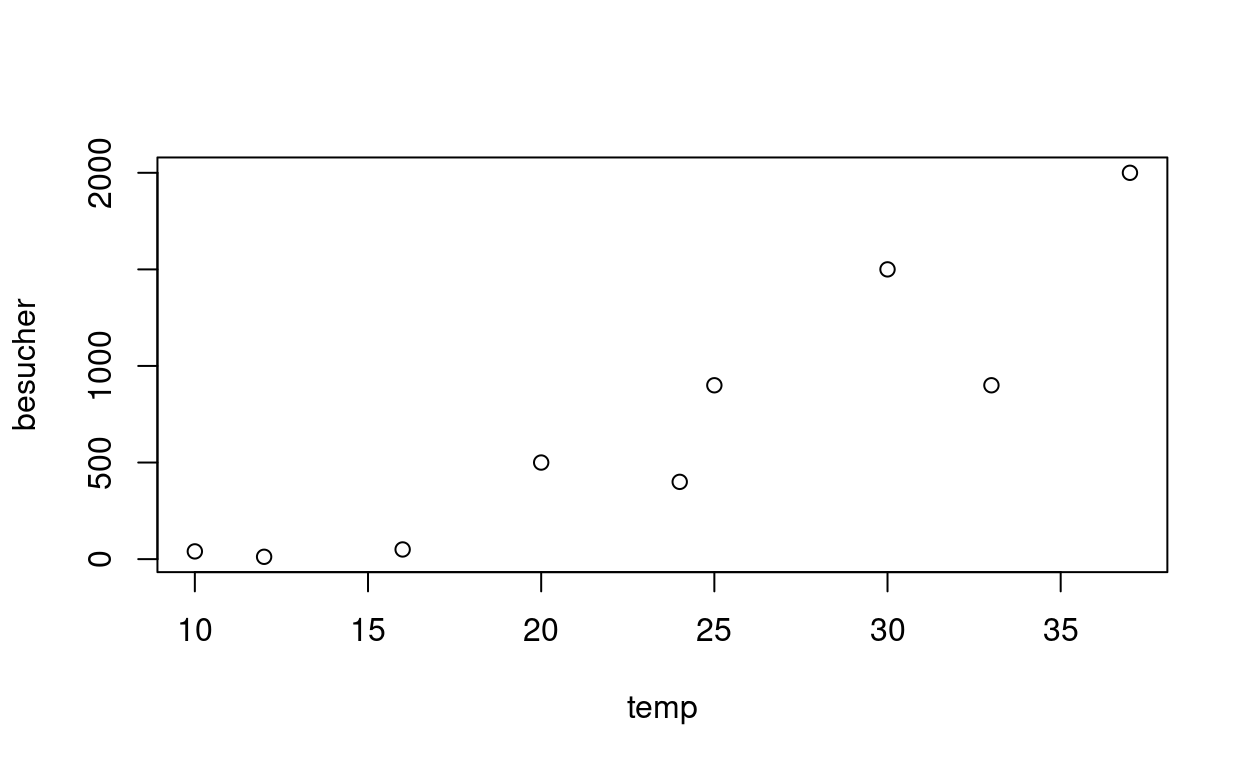
\includegraphics{solution_stat_Beispiel_files/figure-latex/unnamed-chunk-2-1.pdf}

\begin{Shaded}
\begin{Highlighting}[]
\FunctionTok{boxplot}\NormalTok{(decay}\SpecialCharTok{$}\NormalTok{amount)}
\end{Highlighting}
\end{Shaded}

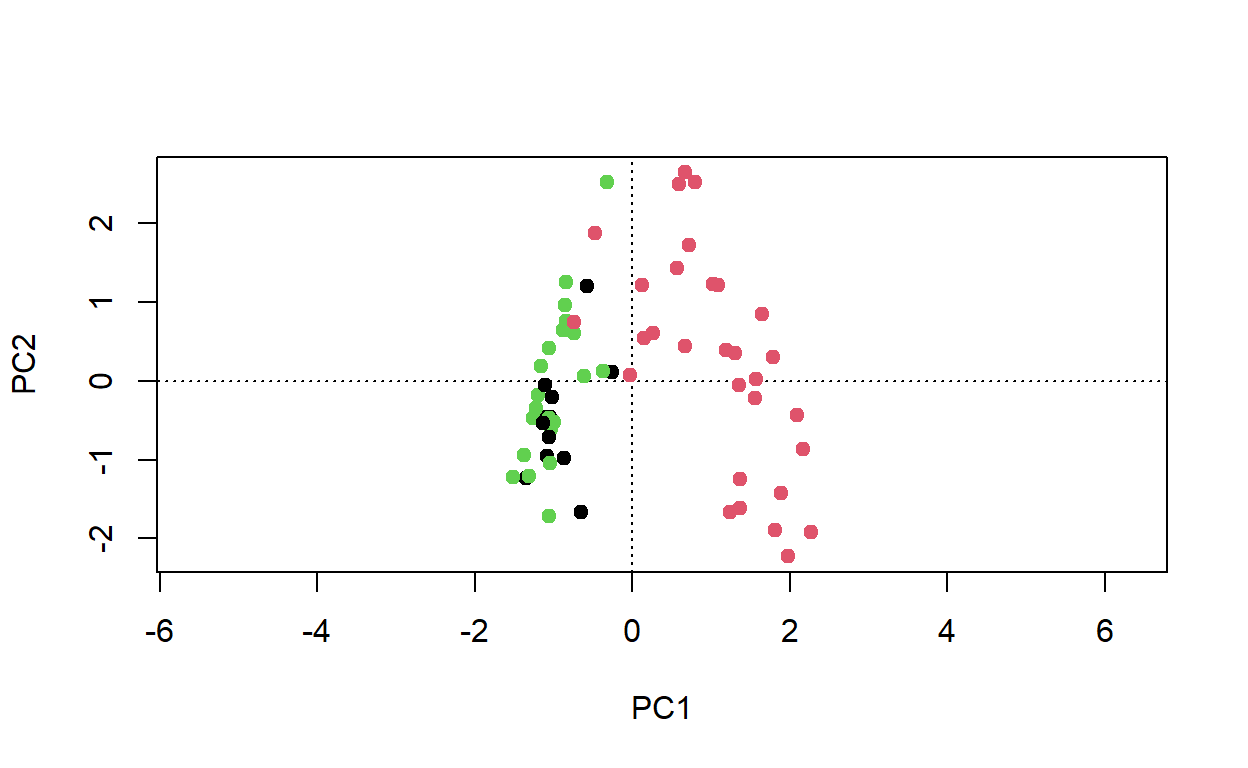
\includegraphics{solution_stat_Beispiel_files/figure-latex/unnamed-chunk-2-2.pdf}

\begin{Shaded}
\begin{Highlighting}[]
\FunctionTok{plot}\NormalTok{(amount}\SpecialCharTok{\textasciitilde{}}\NormalTok{time, }\AttributeTok{data=}\NormalTok{decay)}
\end{Highlighting}
\end{Shaded}

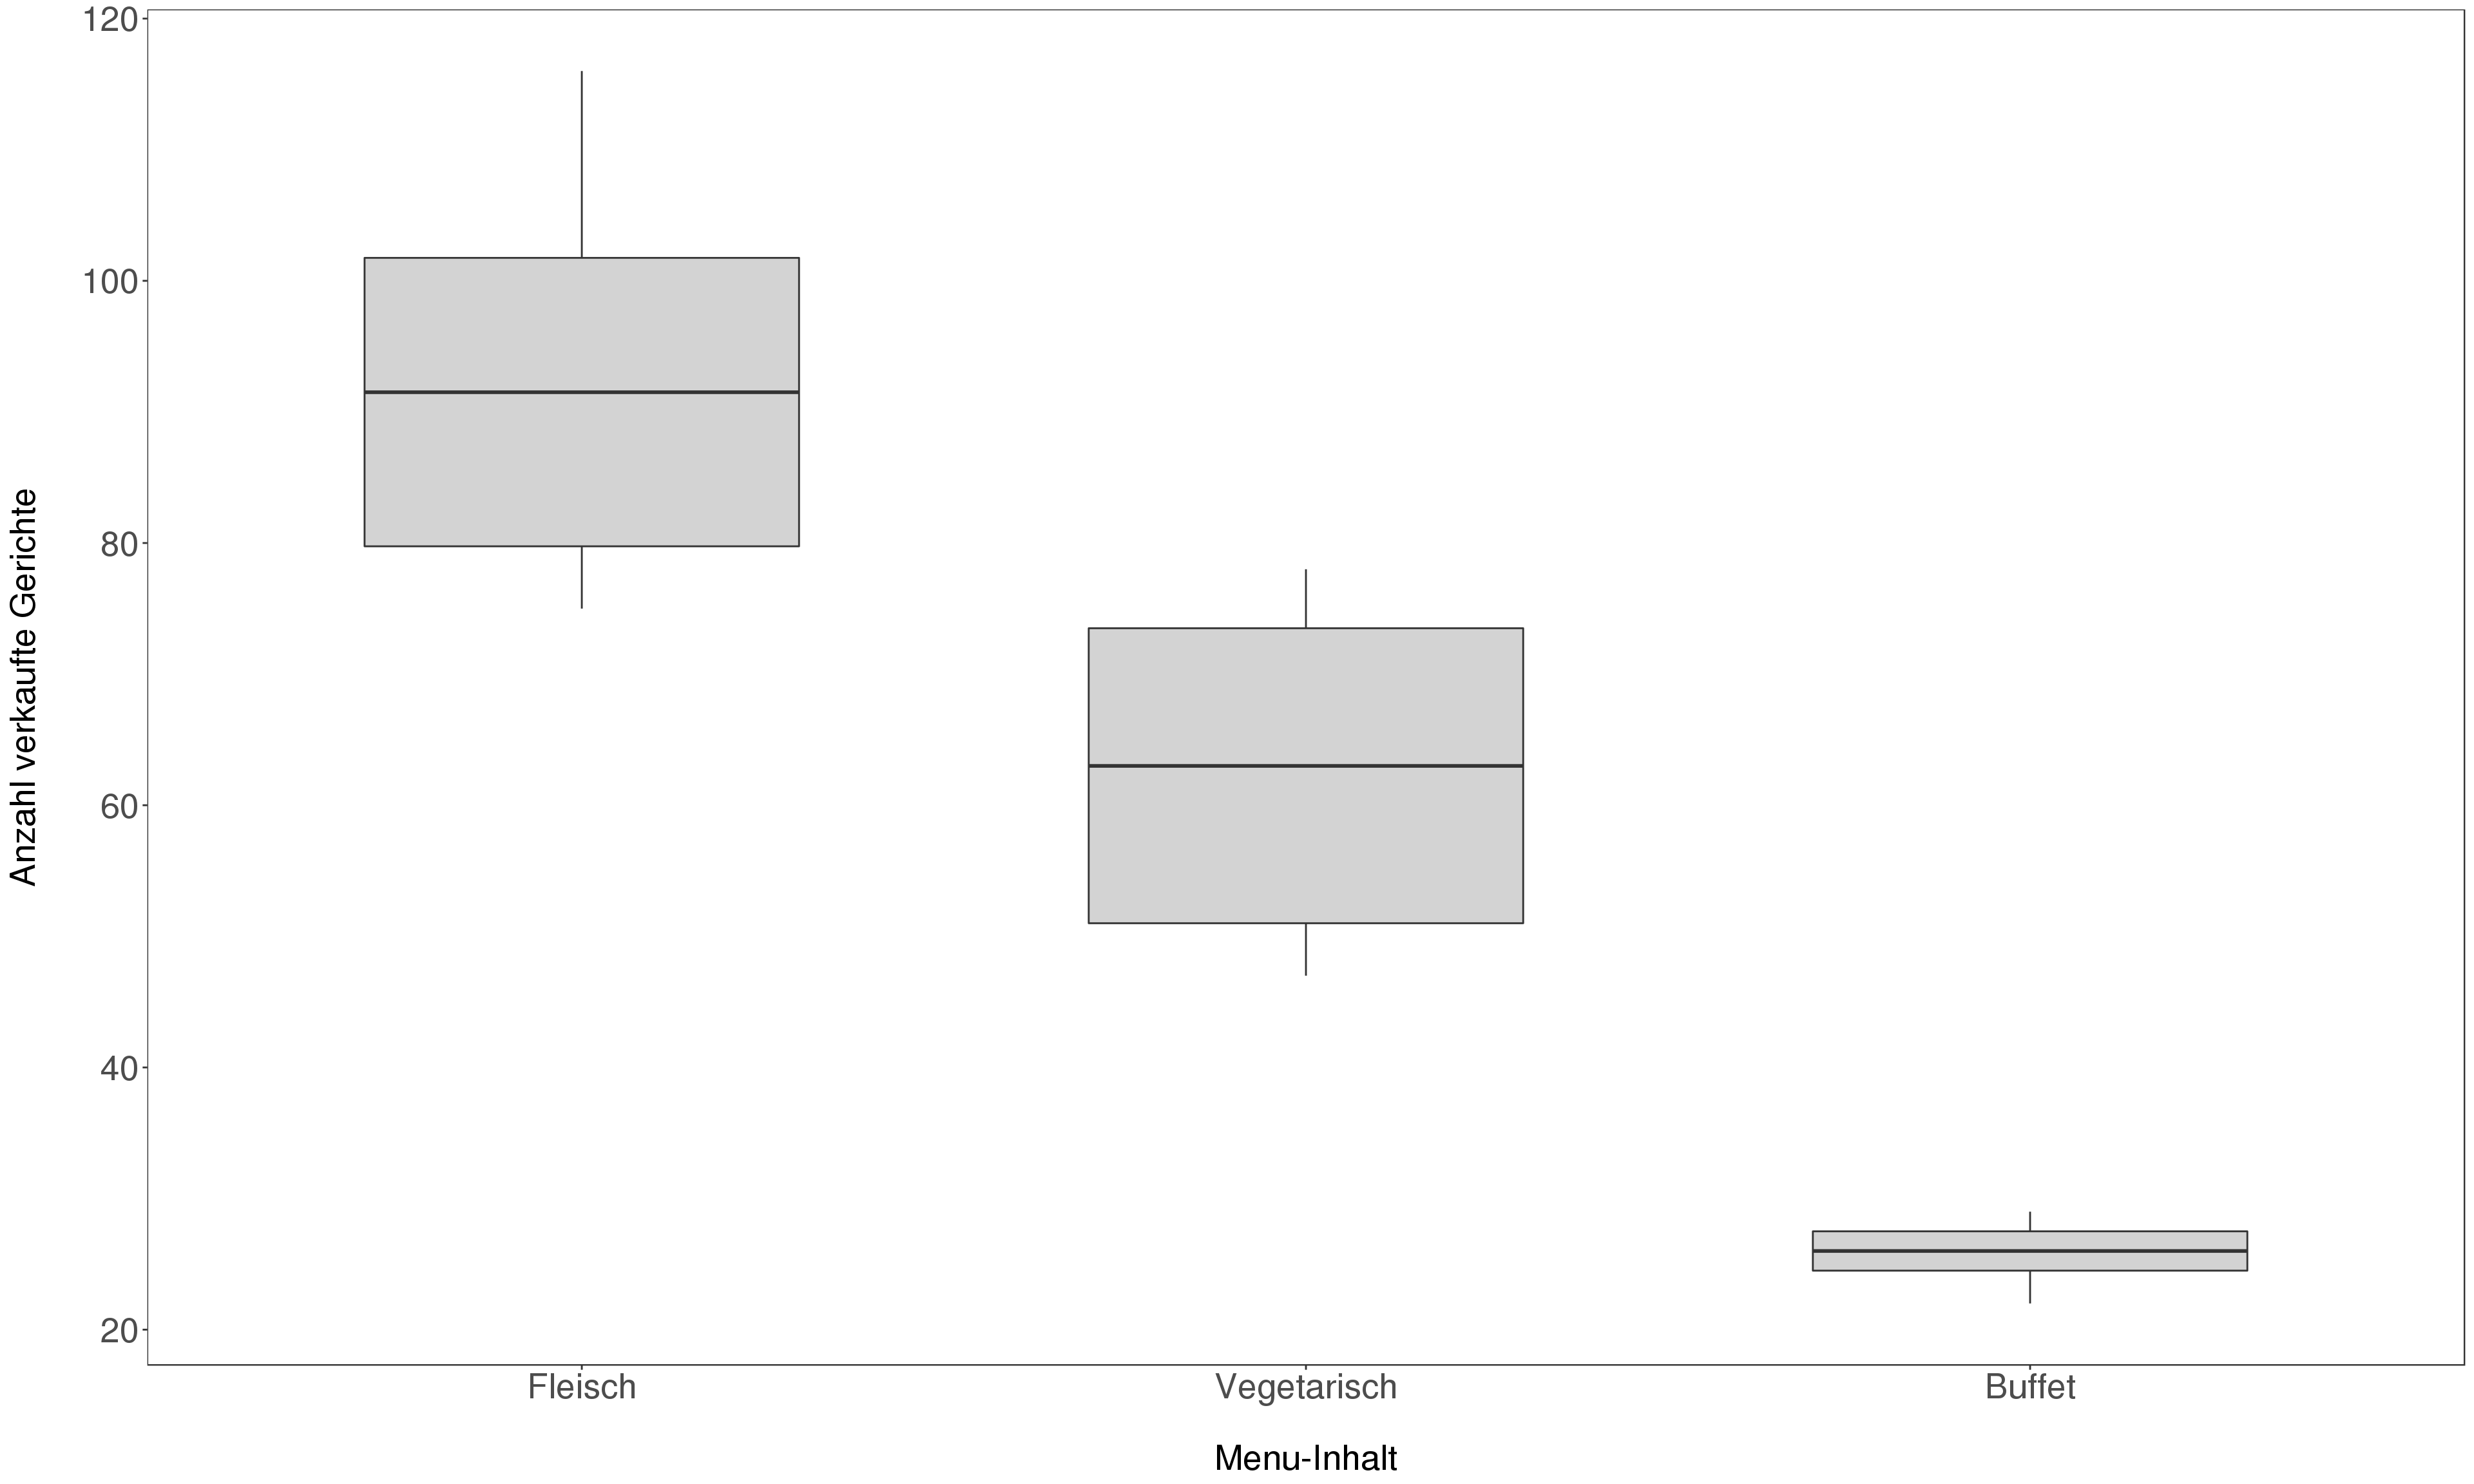
\includegraphics{solution_stat_Beispiel_files/figure-latex/unnamed-chunk-2-3.pdf}

Während der Boxplot für time wunderbar symmetrisch ohne Ausreisser ist,
zeigt amount eine stark rechtsschiefe (linkssteile) Verteilung mit einem
Ausreiser. Das deutet schon an, dass ein einfaches lineares Modell
vermutlich die Modellannahmen verletzen wird. Auch der einfache
Scatterplot zeigt, dass ein lineares Modell wohl nicht adäquat ist. Wir
rechnen aber erst einmal weiter.

\textbf{Einfaches lineares Modell}

\begin{Shaded}
\begin{Highlighting}[]
\NormalTok{lm}\FloatTok{.1} \OtherTok{\textless{}{-}} \FunctionTok{lm}\NormalTok{(amount}\SpecialCharTok{\textasciitilde{}}\NormalTok{time, }\AttributeTok{data=}\NormalTok{decay)}
\FunctionTok{summary}\NormalTok{(lm}\FloatTok{.1}\NormalTok{)}
\end{Highlighting}
\end{Shaded}

\begin{verbatim}
## 
## Call:
## lm(formula = amount ~ time, data = decay)
## 
## Residuals:
##     Min      1Q  Median      3Q     Max 
## -19.065 -10.029  -2.058   5.107  40.447 
## 
## Coefficients:
##             Estimate Std. Error t value Pr(>|t|)    
## (Intercept)  84.5534     5.0277   16.82  < 2e-16 ***
## time         -2.8272     0.2879   -9.82 9.94e-11 ***
## ---
## Signif. codes:  0 '***' 0.001 '**' 0.01 '*' 0.05 '.' 0.1 ' ' 1
## 
## Residual standard error: 14.34 on 29 degrees of freedom
## Multiple R-squared:  0.7688, Adjusted R-squared:  0.7608 
## F-statistic: 96.44 on 1 and 29 DF,  p-value: 9.939e-11
\end{verbatim}

Das sieht erst einmal nach einem Supermodell aus, höchstsignifikant und
mit einem hohen R² von fast 77\%. ABER: wir müssen uns noch die
Modelldiagnostik ansehen\ldots{}

\textbf{Modelldiagnostik}

\begin{Shaded}
\begin{Highlighting}[]
\FunctionTok{par}\NormalTok{(}\AttributeTok{mfrow=}\FunctionTok{c}\NormalTok{(}\DecValTok{2}\NormalTok{,}\DecValTok{2}\NormalTok{))}
\FunctionTok{plot}\NormalTok{(lm}\FloatTok{.1}\NormalTok{)}
\end{Highlighting}
\end{Shaded}

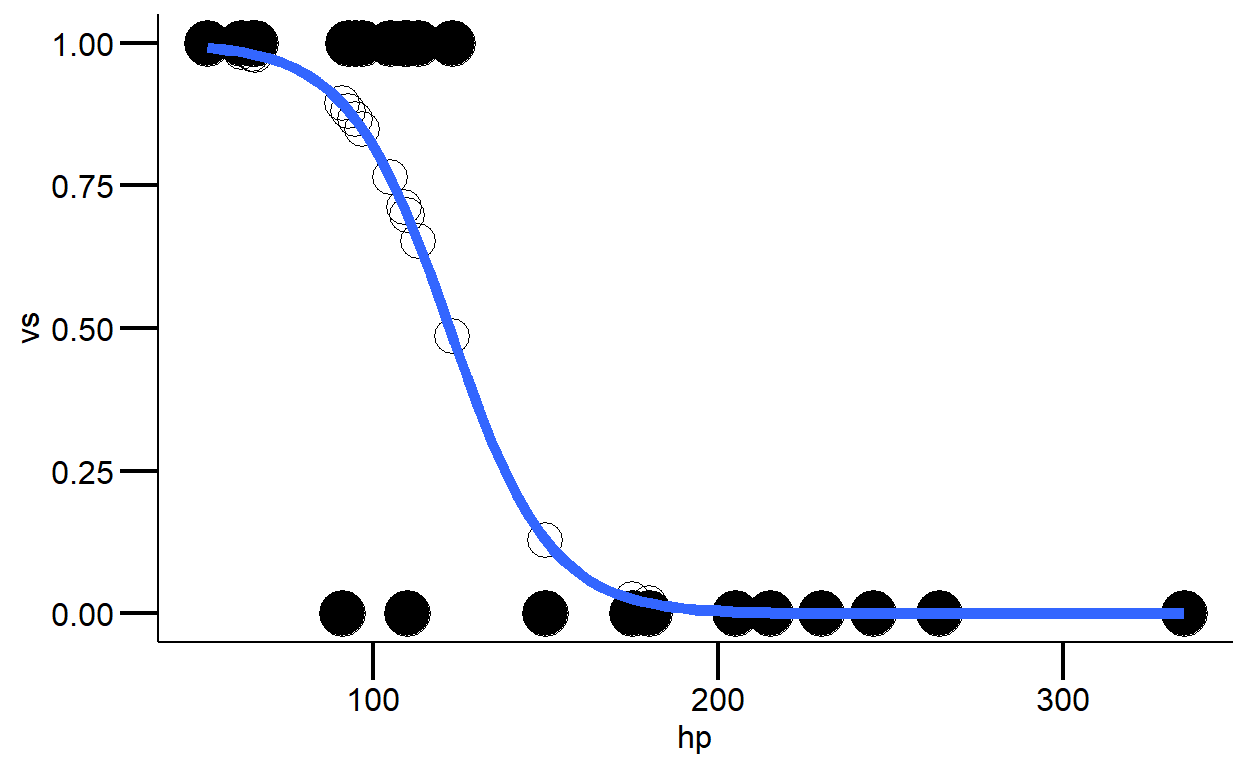
\includegraphics{solution_stat_Beispiel_files/figure-latex/unnamed-chunk-4-1.pdf}
Hier zeigen die wichtigen oberen Plots beide massive Abweichungen vom
„Soll``. Der Plot oben links zeigt eine „Banane`` und beim Q-Q-Plot oben
rechts weichen die Punkte rechts der Mitte alle stark nach oben von der
Solllinie ab. Wir haben unser Modell also offensichtlich falsch
spezifiziert. Um eine Idee zu bekommen, was falsch ist, plotten wir
noch, wie das Ergebnis dieses Modells aussähe:

\textbf{Ergebnisplot}

\begin{Shaded}
\begin{Highlighting}[]
\FunctionTok{par}\NormalTok{(}\AttributeTok{mfrow=}\FunctionTok{c}\NormalTok{(}\DecValTok{1}\NormalTok{,}\DecValTok{1}\NormalTok{))}
\FunctionTok{plot}\NormalTok{(decay}\SpecialCharTok{$}\NormalTok{time, decay}\SpecialCharTok{$}\NormalTok{amount)}
\FunctionTok{abline}\NormalTok{(lm}\FloatTok{.1}\NormalTok{, }\AttributeTok{col=}\StringTok{"red"}\NormalTok{)}
\end{Highlighting}
\end{Shaded}

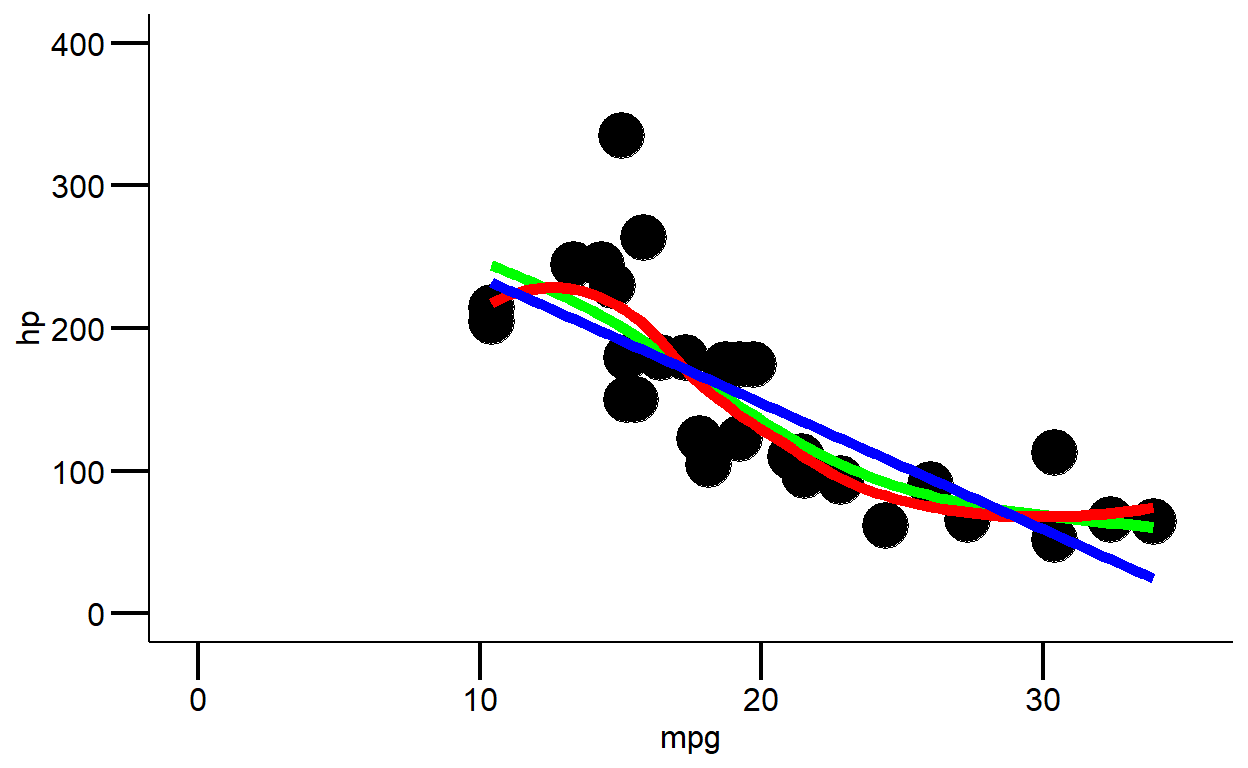
\includegraphics{solution_stat_Beispiel_files/figure-latex/unnamed-chunk-5-1.pdf}

Die Punkte links liegen alle über der Regressionslinie, die in der Mitte
darunter und die ganz rechts wieder systematisch darüber (darum im
Diagnostikplot oben die „Banane``). Es liegt also offensichtlich keine
lineare Beziehung vor, sondern eine curvilineare.

Um diese korrekt zu analysieren, gibt es im Prinzip drei Möglichkeiten,
wovon am zweiten Kurstag nur eine hatten, während die zweite und dritte
in Statistik 3 und 4 folgten. Im Folgenden sind alle drei nacheinander
dargestellt (in der Klausur würde es aber genügen, eine davon
darzustellen, wenn die Aufgabenstellung wie oben lautet).

\textbf{Variante (1): Lineares Modell nach Transformation der abhängigen
Variablen} Dass die Verteilung der abhängigen Variable nicht normal ist,
haben wir ja schon bei der explorativen Datenanalyse am Anfang gesehen.
Da sie stark linkssteil ist, zugleich aber keine Nullwerte enthält,
bietet sich eine Logarithmustransformation an, hier z. B. mit dem
natürlichen Logarithmus.

\textbf{Loesung 1: log-Transformation der abhaengigen Variablen}

\begin{Shaded}
\begin{Highlighting}[]
\FunctionTok{par}\NormalTok{(}\AttributeTok{mfrow=}\FunctionTok{c}\NormalTok{(}\DecValTok{1}\NormalTok{,}\DecValTok{2}\NormalTok{))}
\FunctionTok{boxplot}\NormalTok{(decay}\SpecialCharTok{$}\NormalTok{amount)}
\FunctionTok{boxplot}\NormalTok{(}\FunctionTok{log}\NormalTok{(decay}\SpecialCharTok{$}\NormalTok{amount))}
\end{Highlighting}
\end{Shaded}

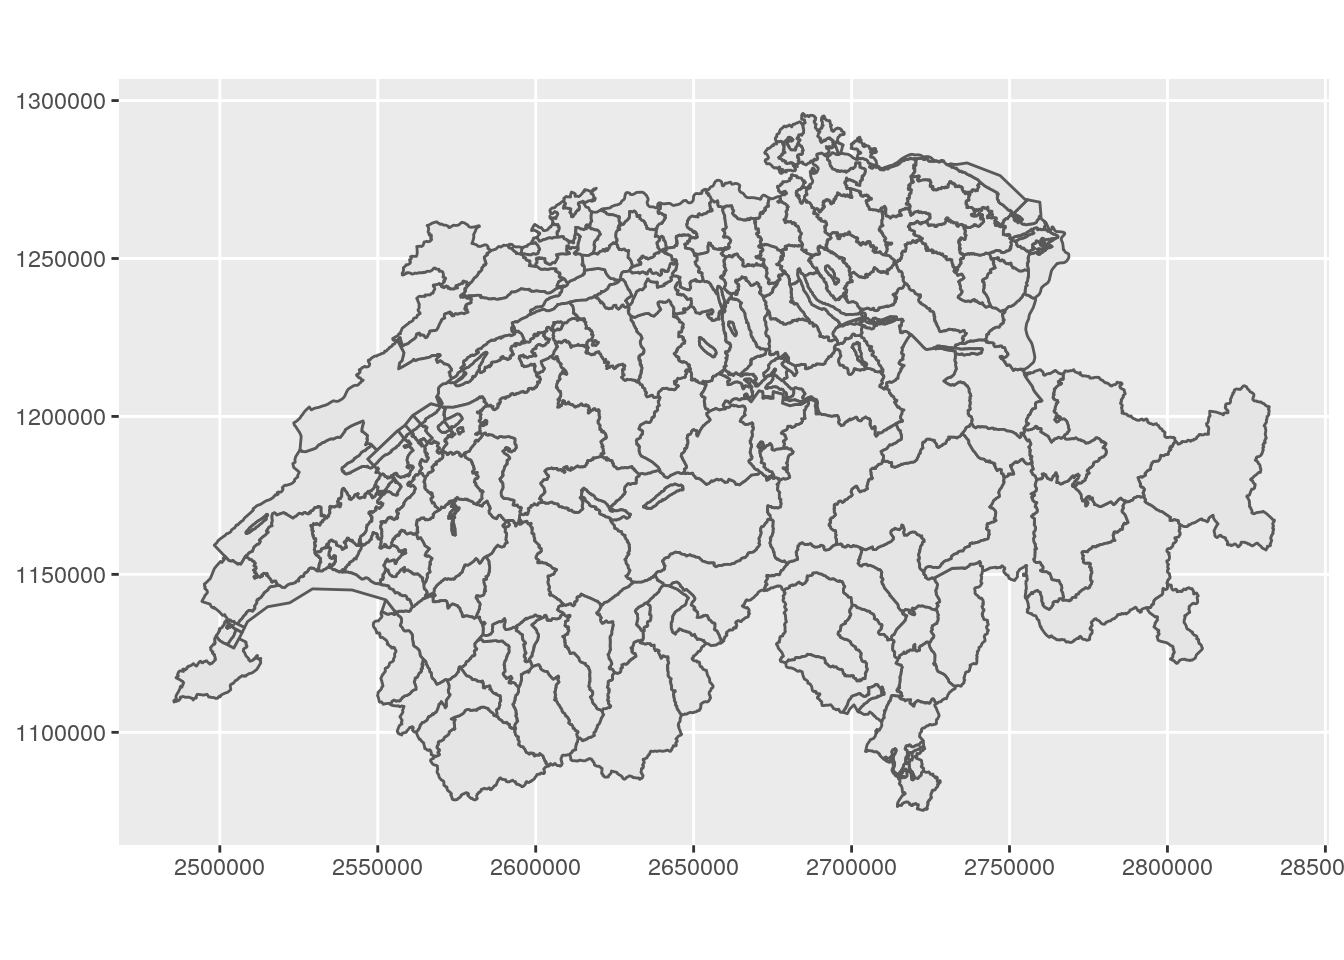
\includegraphics{solution_stat_Beispiel_files/figure-latex/unnamed-chunk-6-1.pdf}

\begin{Shaded}
\begin{Highlighting}[]
\FunctionTok{hist}\NormalTok{(decay}\SpecialCharTok{$}\NormalTok{amount)}
\FunctionTok{hist}\NormalTok{(}\FunctionTok{log}\NormalTok{(decay}\SpecialCharTok{$}\NormalTok{amount))}
\end{Highlighting}
\end{Shaded}

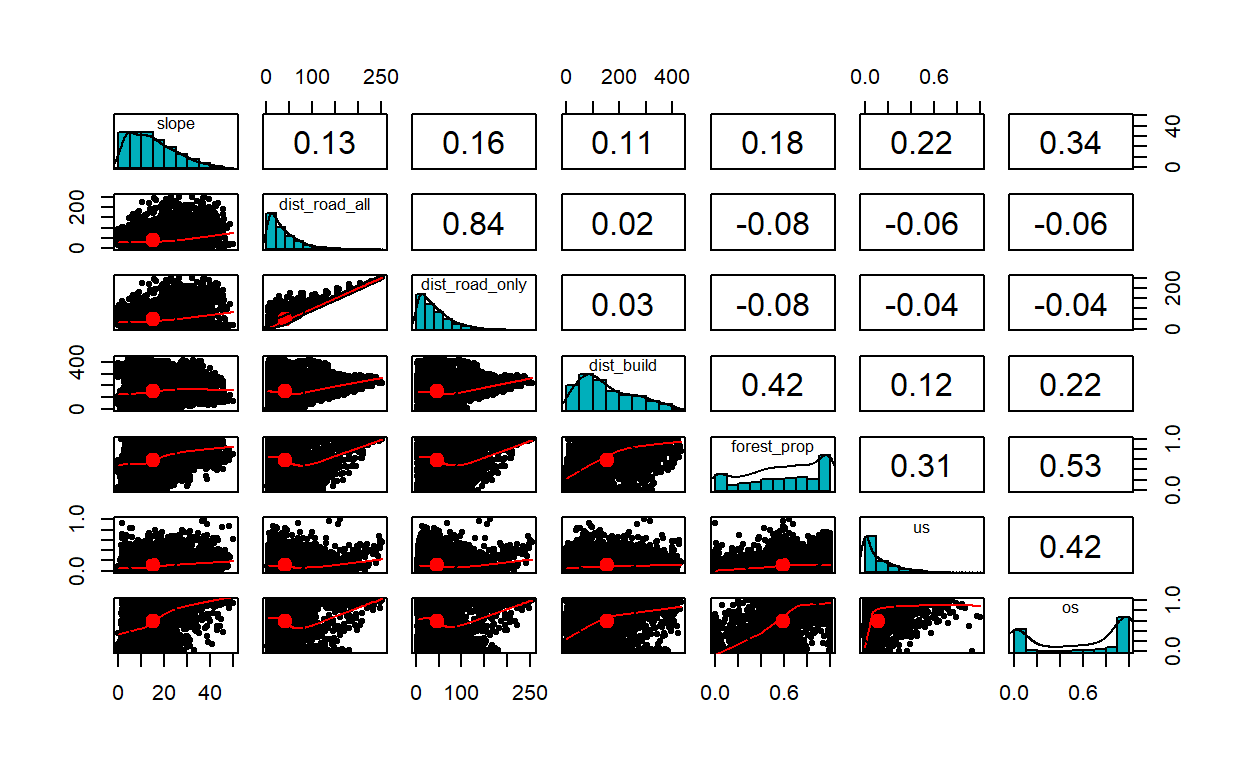
\includegraphics{solution_stat_Beispiel_files/figure-latex/unnamed-chunk-6-2.pdf}
\#Die log-transformierte Variante rechts sieht sowohl im Boxplot als
auch im \#Histogramm viel symmetrischer/besser normalverteilt aus. Damit
ergibt sich \#dann folgendes lineares Modell

\begin{Shaded}
\begin{Highlighting}[]
\NormalTok{lm}\FloatTok{.2} \OtherTok{\textless{}{-}} \FunctionTok{lm}\NormalTok{(}\FunctionTok{log}\NormalTok{(amount)}\SpecialCharTok{\textasciitilde{}}\NormalTok{time, }\AttributeTok{data=}\NormalTok{decay)}
\FunctionTok{summary}\NormalTok{(lm}\FloatTok{.2}\NormalTok{)}
\end{Highlighting}
\end{Shaded}

\begin{verbatim}
## 
## Call:
## lm(formula = log(amount) ~ time, data = decay)
## 
## Residuals:
##     Min      1Q  Median      3Q     Max 
## -0.5935 -0.2043  0.0067  0.2198  0.6297 
## 
## Coefficients:
##              Estimate Std. Error t value Pr(>|t|)    
## (Intercept)  4.547386   0.100295   45.34  < 2e-16 ***
## time        -0.068528   0.005743  -11.93 1.04e-12 ***
## ---
## Signif. codes:  0 '***' 0.001 '**' 0.01 '*' 0.05 '.' 0.1 ' ' 1
## 
## Residual standard error: 0.286 on 29 degrees of freedom
## Multiple R-squared:  0.8308, Adjusted R-squared:  0.825 
## F-statistic: 142.4 on 1 and 29 DF,  p-value: 1.038e-12
\end{verbatim}

Jetzt ist der R²-Wert noch höher und der p-Wert noch niedriger als im
ursprünglichen linearen Modell ohne Transformation. Das erlaubt aber
keine Aussage, da wir Äpfel mit Birnen vergleichen, da die abhängige
Variable einmal untransformiert und einmal log-transformiert ist.
Entscheidend ist die Modelldiagnostik.

\textbf{Modelldiagnostik}

\begin{Shaded}
\begin{Highlighting}[]
\FunctionTok{par}\NormalTok{(}\AttributeTok{mfrow=}\FunctionTok{c}\NormalTok{(}\DecValTok{2}\NormalTok{,}\DecValTok{2}\NormalTok{))}
\FunctionTok{plot}\NormalTok{(lm}\FloatTok{.2}\NormalTok{)}
\end{Highlighting}
\end{Shaded}

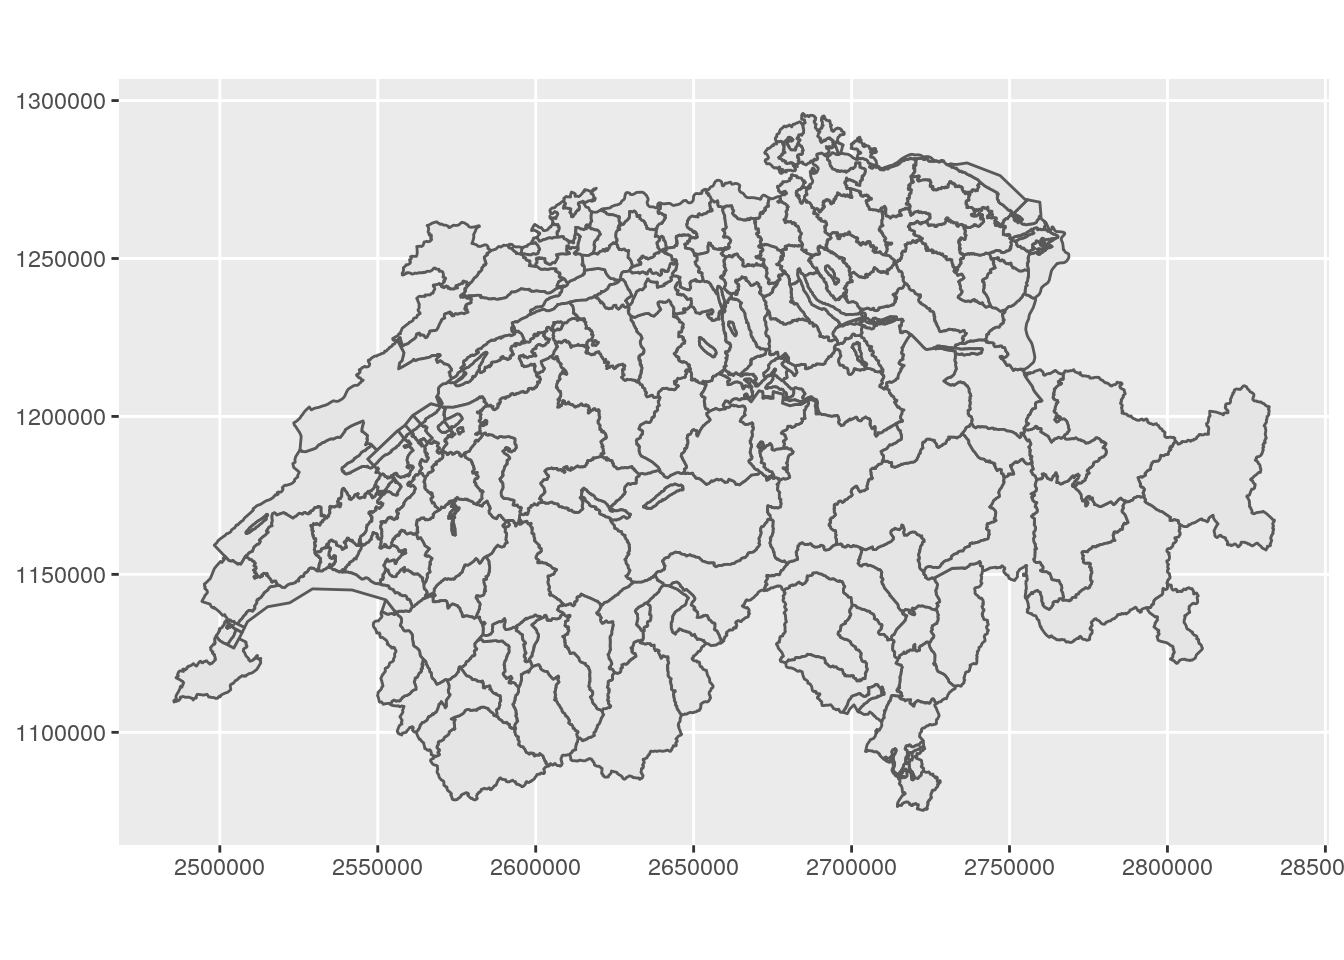
\includegraphics{solution_stat_Beispiel_files/figure-latex/unnamed-chunk-8-1.pdf}

Der Q-Q-Plot sieht jetzt exzellent aus, der Plot rechts oben hat kaum
noch eine Banane, nur noch einen leichten Keil. Insgesamt deutlich
besser und auf jeden Fall ein statistisch korrektes Modell.

Lösungen 2 und 3 greifen auf Methoden von Statistik 3 und 4 zurück, sie
sind hier nur zum Vergleich angeführt

\textbf{Loesung 2: quadratische Regression (kam erst in Statistik 3;}
\emph{\textbf{koente fuer die Datenverteilung passen, entspricht aber
nicht der physikalischen}}

\textbf{Gesetzmaessigkeit}

\begin{Shaded}
\begin{Highlighting}[]
\NormalTok{model.quad }\OtherTok{\textless{}{-}} \FunctionTok{lm}\NormalTok{(amount}\SpecialCharTok{\textasciitilde{}}\NormalTok{time}\SpecialCharTok{+}\FunctionTok{I}\NormalTok{(time}\SpecialCharTok{\^{}}\DecValTok{2}\NormalTok{), }\AttributeTok{data=}\NormalTok{decay)}
\FunctionTok{summary}\NormalTok{(model.quad)}
\end{Highlighting}
\end{Shaded}

\begin{verbatim}
## 
## Call:
## lm(formula = amount ~ time + I(time^2), data = decay)
## 
## Residuals:
##     Min      1Q  Median      3Q     Max 
## -22.302  -6.044  -1.603   4.224  20.581 
## 
## Coefficients:
##              Estimate Std. Error t value Pr(>|t|)    
## (Intercept) 106.38880    4.65627  22.849  < 2e-16 ***
## time         -7.34485    0.71844 -10.223 5.90e-11 ***
## I(time^2)     0.15059    0.02314   6.507 4.73e-07 ***
## ---
## Signif. codes:  0 '***' 0.001 '**' 0.01 '*' 0.05 '.' 0.1 ' ' 1
## 
## Residual standard error: 9.205 on 28 degrees of freedom
## Multiple R-squared:  0.908,  Adjusted R-squared:  0.9014 
## F-statistic: 138.1 on 2 and 28 DF,  p-value: 3.122e-15
\end{verbatim}

Hier können wir R² mit dem ursprünglichen Modell vergleichen (beide
haben amount als abhängige Grösse) und es sieht viel besser aus. Sowohl
der lineare als auch der quadratische Term sind hochsignifikant.
Sicherheitshalber vergleichen wir die beiden Modelle aber noch mittels
ANOVA.

\textbf{Vergleich mit dem einfachen Modell mittels ANOVA (es ginge auch
AICc)}

\begin{Shaded}
\begin{Highlighting}[]
\FunctionTok{anova}\NormalTok{(lm}\FloatTok{.1}\NormalTok{, model.quad)}
\end{Highlighting}
\end{Shaded}

\begin{verbatim}
## Analysis of Variance Table
## 
## Model 1: amount ~ time
## Model 2: amount ~ time + I(time^2)
##   Res.Df    RSS Df Sum of Sq      F    Pr(>F)    
## 1     29 5960.6                                  
## 2     28 2372.6  1    3588.1 42.344 4.727e-07 ***
## ---
## Signif. codes:  0 '***' 0.001 '**' 0.01 '*' 0.05 '.' 0.1 ' ' 1
\end{verbatim}

In der Tat ist das komplexere Modell (jenes mit dem quadratischen Term)
höchstsignifikant besser. Jetzt brauchen wir noch die Modelldiagnostik.

\textbf{Modelldiagnostik}

\begin{Shaded}
\begin{Highlighting}[]
\FunctionTok{par}\NormalTok{(}\AttributeTok{mfrow=}\FunctionTok{c}\NormalTok{(}\DecValTok{2}\NormalTok{,}\DecValTok{2}\NormalTok{))}
\FunctionTok{plot}\NormalTok{(model.quad)}
\end{Highlighting}
\end{Shaded}

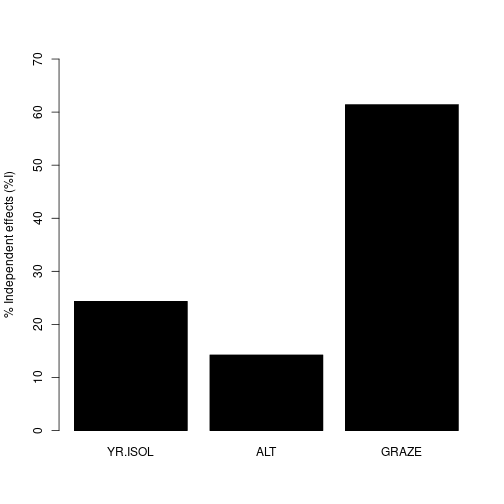
\includegraphics{solution_stat_Beispiel_files/figure-latex/unnamed-chunk-11-1.pdf}

\textbf{Loesung 3 (die beste, hatten wir aber am 2. Tag noch nicht; mit
Startwerten muss man ggf. ausprobieren)}

\emph{\textbf{mit Startwerten muss man ggf. ausprobieren)}}

\begin{Shaded}
\begin{Highlighting}[]
\NormalTok{model.nls }\OtherTok{\textless{}{-}} \FunctionTok{nls}\NormalTok{(amount}\SpecialCharTok{\textasciitilde{}}\NormalTok{a}\SpecialCharTok{*}\FunctionTok{exp}\NormalTok{(}\SpecialCharTok{{-}}\NormalTok{b}\SpecialCharTok{*}\NormalTok{time), }\AttributeTok{start=}\NormalTok{(}\FunctionTok{list}\NormalTok{(}\AttributeTok{a=}\DecValTok{100}\NormalTok{,}\AttributeTok{b=}\DecValTok{1}\NormalTok{)),}\AttributeTok{data=}\NormalTok{decay)}
\FunctionTok{summary}\NormalTok{(model.nls)}
\end{Highlighting}
\end{Shaded}

\begin{verbatim}
## 
## Formula: amount ~ a * exp(-b * time)
## 
## Parameters:
##    Estimate Std. Error t value Pr(>|t|)    
## a 1.081e+02  4.993e+00   21.66  < 2e-16 ***
## b 8.019e-02  5.833e-03   13.75 3.12e-14 ***
## ---
## Signif. codes:  0 '***' 0.001 '**' 0.01 '*' 0.05 '.' 0.1 ' ' 1
## 
## Residual standard error: 9.243 on 29 degrees of freedom
## 
## Number of iterations to convergence: 8 
## Achieved convergence tolerance: 7.966e-06
\end{verbatim}

\textbf{Modelldiagnostik}

\begin{Shaded}
\begin{Highlighting}[]
\ControlFlowTok{if}\NormalTok{(}\SpecialCharTok{!}\FunctionTok{require}\NormalTok{(nlstools))\{}\FunctionTok{install.packages}\NormalTok{(}\StringTok{"nlstools"}\NormalTok{)\}}
\end{Highlighting}
\end{Shaded}

\begin{verbatim}
## Loading required package: nlstools
\end{verbatim}

\begin{verbatim}
## 
## 'nlstools' has been loaded.
\end{verbatim}

\begin{verbatim}
## IMPORTANT NOTICE: Most nonlinear regression models and data set examples
\end{verbatim}

\begin{verbatim}
## related to predictive microbiolgy have been moved to the package 'nlsMicrobio'
\end{verbatim}

\begin{Shaded}
\begin{Highlighting}[]
\FunctionTok{library}\NormalTok{(nlstools)}
\NormalTok{residuals.nls }\OtherTok{\textless{}{-}} \FunctionTok{nlsResiduals}\NormalTok{(model.nls)}
\FunctionTok{plot}\NormalTok{(residuals.nls)}
\end{Highlighting}
\end{Shaded}

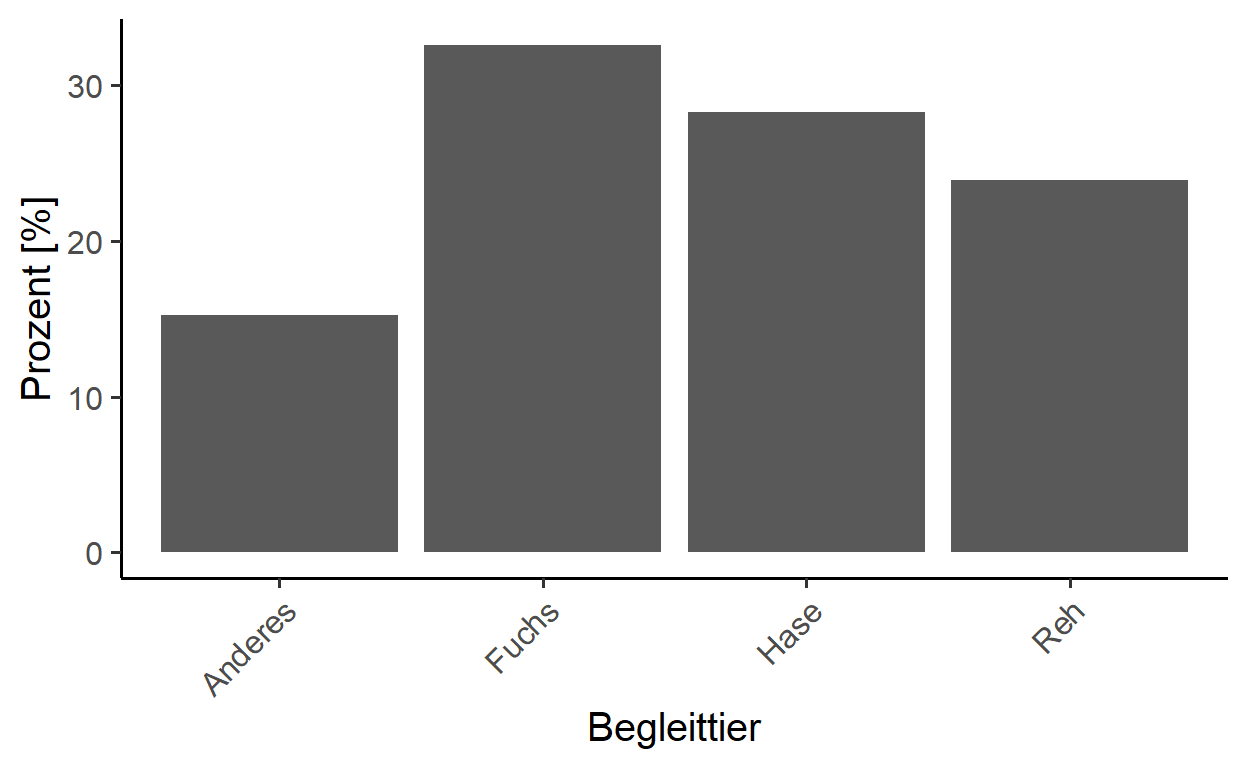
\includegraphics{solution_stat_Beispiel_files/figure-latex/unnamed-chunk-13-1.pdf}

Für nls kann man nicht den normalen Plotbefehl für die
Residualdiagnostik nehmen, sondern verwendet das Äquivalent aus
nlstools. Die beiden entscheidenden Plots sind jetzt links oben und
rechts unten. Der QQ-Plot hat im unteren Bereich einen kleinen
Schönheitsfehler, aber ansonsten ist alles OK.

Da alle drei Lösungen zumindest statistisch OK waren, sollen jetzt noch
die zugehörigen Ergebnisplots erstellt werden.

\textbf{Ergebnisplots}

\begin{Shaded}
\begin{Highlighting}[]
\FunctionTok{par}\NormalTok{(}\AttributeTok{mfrow=}\FunctionTok{c}\NormalTok{(}\DecValTok{1}\NormalTok{,}\DecValTok{1}\NormalTok{))}
\NormalTok{xv }\OtherTok{\textless{}{-}} \FunctionTok{seq}\NormalTok{(}\DecValTok{0}\NormalTok{,}\DecValTok{30}\NormalTok{,}\FloatTok{0.1}\NormalTok{)}
\end{Highlighting}
\end{Shaded}

\begin{enumerate}
\def\labelenumi{\arabic{enumi}.}
\tightlist
\item
  lineares Modell mit log-transformierter Abhaengiger
\end{enumerate}

\begin{Shaded}
\begin{Highlighting}[]
\FunctionTok{plot}\NormalTok{(decay}\SpecialCharTok{$}\NormalTok{time, decay}\SpecialCharTok{$}\NormalTok{amount)}
\NormalTok{yv1 }\OtherTok{\textless{}{-}} \FunctionTok{exp}\NormalTok{(}\FunctionTok{predict}\NormalTok{(lm}\FloatTok{.2}\NormalTok{, }\FunctionTok{list}\NormalTok{(}\AttributeTok{time=}\NormalTok{xv)))}
\FunctionTok{lines}\NormalTok{(xv, yv1, }\AttributeTok{col=}\StringTok{"red"}\NormalTok{)}
\end{Highlighting}
\end{Shaded}

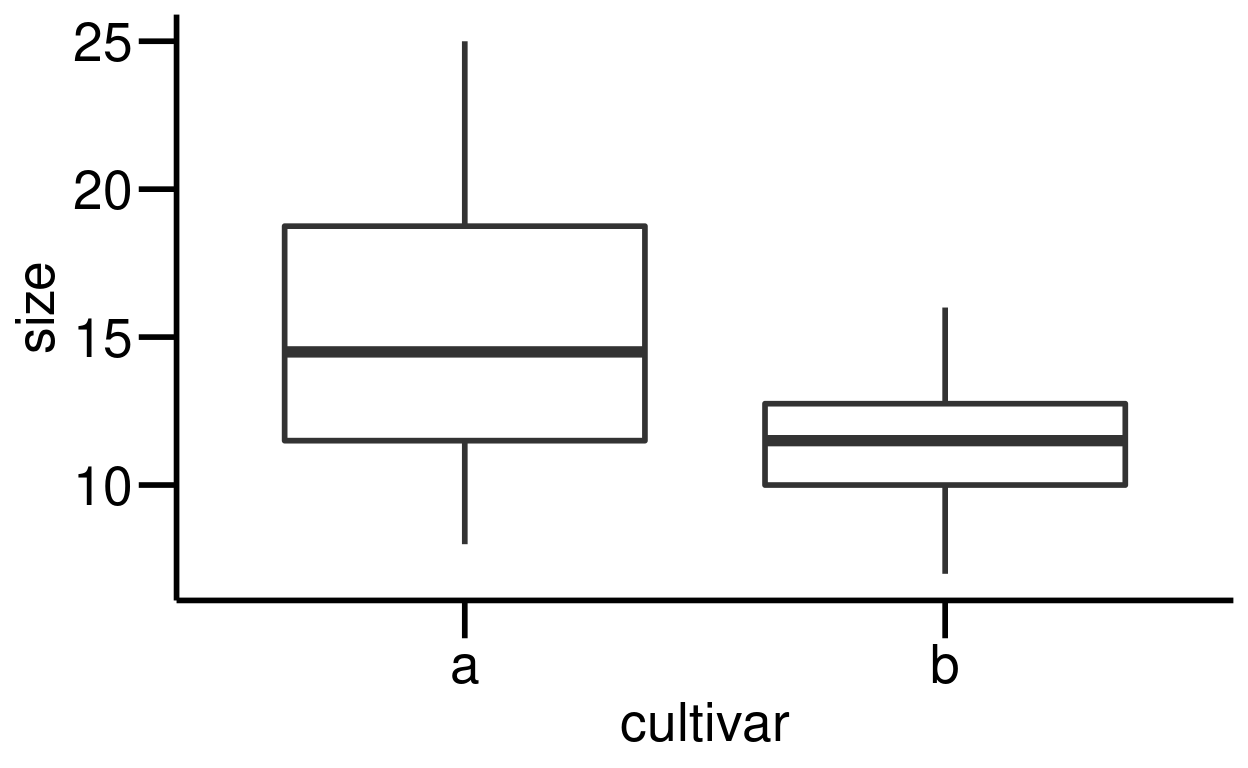
\includegraphics{solution_stat_Beispiel_files/figure-latex/unnamed-chunk-15-1.pdf}

\begin{enumerate}
\def\labelenumi{\arabic{enumi}.}
\setcounter{enumi}{1}
\tightlist
\item
  quadratisches Modell
\end{enumerate}

\begin{Shaded}
\begin{Highlighting}[]
\FunctionTok{plot}\NormalTok{(decay}\SpecialCharTok{$}\NormalTok{time, decay}\SpecialCharTok{$}\NormalTok{amount)}
\NormalTok{yv2 }\OtherTok{\textless{}{-}} \FunctionTok{predict}\NormalTok{(model.quad, }\FunctionTok{list}\NormalTok{(}\AttributeTok{time=}\NormalTok{xv))}
\FunctionTok{lines}\NormalTok{(xv, yv2, }\AttributeTok{col=}\StringTok{"blue"}\NormalTok{)}
\end{Highlighting}
\end{Shaded}

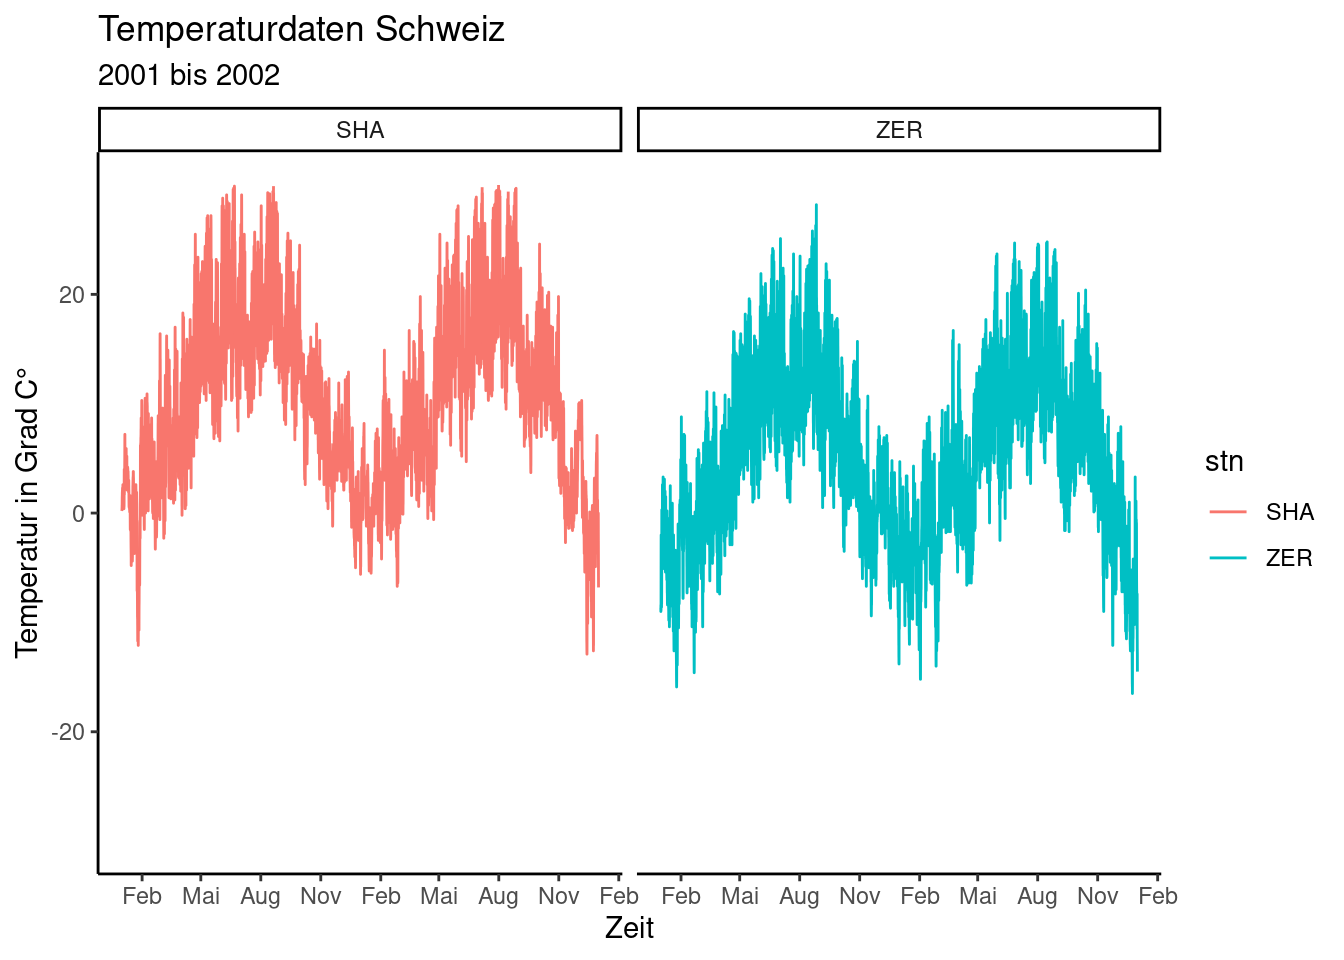
\includegraphics{solution_stat_Beispiel_files/figure-latex/unnamed-chunk-16-1.pdf}

\begin{enumerate}
\def\labelenumi{\arabic{enumi}.}
\setcounter{enumi}{2}
\tightlist
\item
  nicht-lineares Modell
\end{enumerate}

\begin{Shaded}
\begin{Highlighting}[]
\FunctionTok{plot}\NormalTok{(decay}\SpecialCharTok{$}\NormalTok{time, decay}\SpecialCharTok{$}\NormalTok{amount)}
\NormalTok{yv3 }\OtherTok{\textless{}{-}} \FunctionTok{predict}\NormalTok{(model.nls, }\FunctionTok{list}\NormalTok{(}\AttributeTok{time=}\NormalTok{xv))}
\FunctionTok{lines}\NormalTok{(xv, yv3, }\AttributeTok{col=}\StringTok{"green"}\NormalTok{)}
\end{Highlighting}
\end{Shaded}

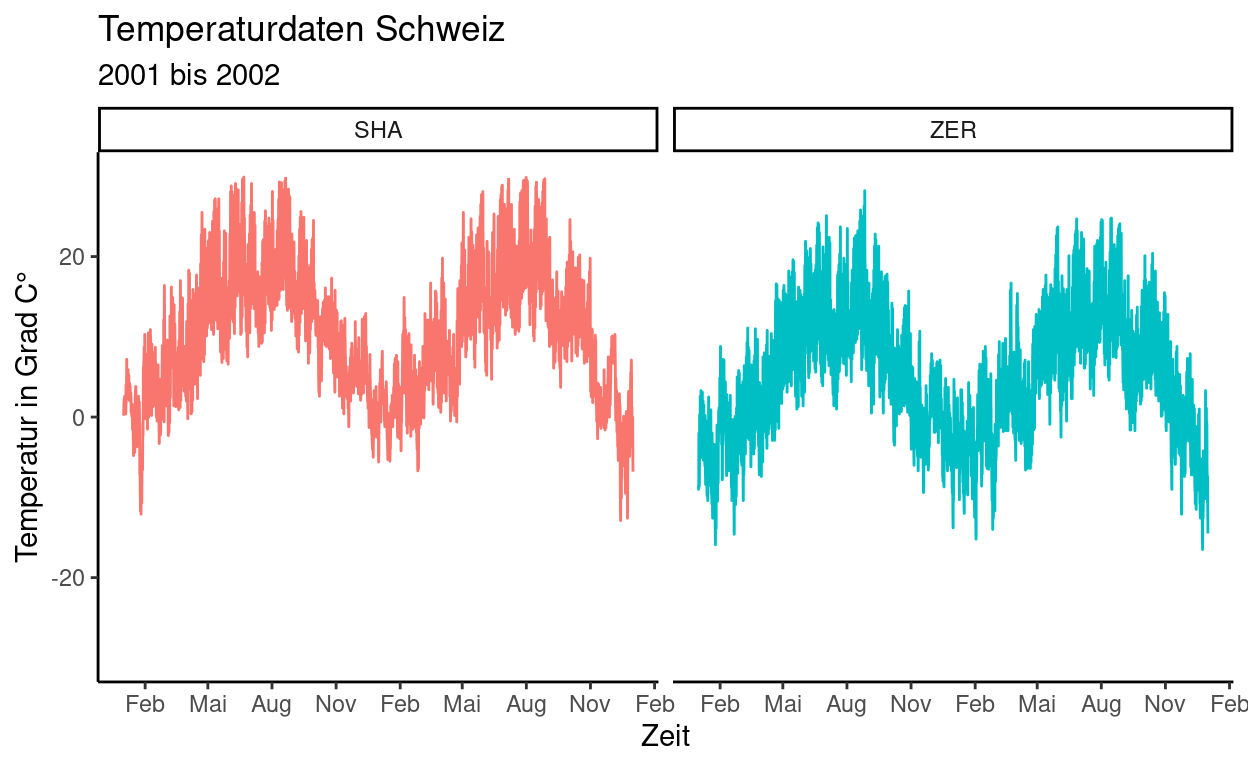
\includegraphics{solution_stat_Beispiel_files/figure-latex/unnamed-chunk-17-1.pdf}
Optisch betrachtet, geben (2) und (3) den empirischen Zusammenhang etwas
besser wieder als (1), da sie im linken Bereich die hohen Werte besser
treffen. Man könnte sogar meinen, bei Betrachtung der Daten, dass die
Werte ab time = 28 wieder leicht ansteigen, was die quadratische
Funktion wiedergibt. Wer sich aber mit Physik etwas auskennt, weiss,
dass Version (2) physikalisch nicht zutrifft, da die Zerfallsrate mit
der Zeit immer weiter abfällt. Aufgrund der kurzen Messreihe wäre eine
quadratische Funktion trotzdem eine statistisch korrekte Interpretation.
Mit längeren Messreihen würde sich jedoch schnell zeigen, dass sie nicht
zutrifft.

\end{document}
